
%(BEGIN_QUESTION)
% Copyright 2014, Tony R. Kuphaldt, released under the Creative Commons Attribution License (v 1.0)
% This means you may do almost anything with this work of mine, so long as you give me proper credit

Disse to reguleringsventilene er split-ranget og styres av samme pneumatiske utgangssignal fra én I/P-transduser. Bench set-området for hver ventil er valgt for å lage riktig split-range-sekvens:

$$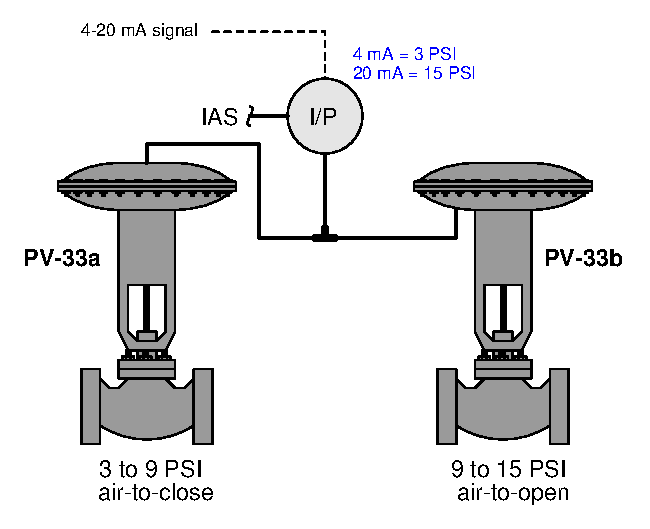
\includegraphics[width=15.5cm]{i00949x01.eps}$$

Beregn ventilposisjon (prosent åpen: 0\% helt stengt, 100\% helt åpen), gitt strømsignal 9 mA til I/P:

\vskip 20pt

\hskip 50pt PV-33a = \underbar{\hskip 50pt} \% åpen \hskip 60pt PV-33b = \underbar{\hskip 50pt} \% åpen

\underbar{file i00949}
%(END_QUESTION)





%(BEGIN_ANSWER)

PV-33a = \underbar{\bf 37.5} \% åpen \hskip 100pt PV-33b = \underbar{\bf 0} \% åpen

%(END_ANSWER)





%(BEGIN_NOTES)

{\bf Denne oppgaven er ment kun for eksamen, ikke for arbeidsark!}.

%(END_NOTES)

